\documentclass[12pt,a4paper]{article}
\usepackage[utf8]{inputenc}
\usepackage[T1]{fontenc}
\usepackage{AMcolor}
\usepackage{pdflscape}
\usepackage[text=tumhlv]{AMfont}
\usepackage[all]{tcolorbox}
\usepackage[paperwidth=30cm,paperheight=6cm,left=3cm,right=6.5cm,top=3cm]{geometry}
\setlength\parindent{0pt}
\pagestyle{empty}

\begin{document}
\begin{tcolorbox}[size=tight,oversize,sharp corners,enhanced,
	colframe=TUMBlue,colback=TUMBlue,colupper=TUMBlue,
	enlarge left by=-100pt,right=260pt,left=30pt,bottom=30pt,top=20pt,
	frame code app={
		\path[tcb fill frame] ([xshift=-2cm]frame.north) to[out=180,in=0] ([xshift=3cm,yshift=60pt]frame.north west)
			-- ([yshift=60pt]frame.north west) -- (frame.north west) --cycle;
	},overlay={%
		\node[black,anchor=east,xshift=-20pt] at ([xshift=-3cm]frame.east) {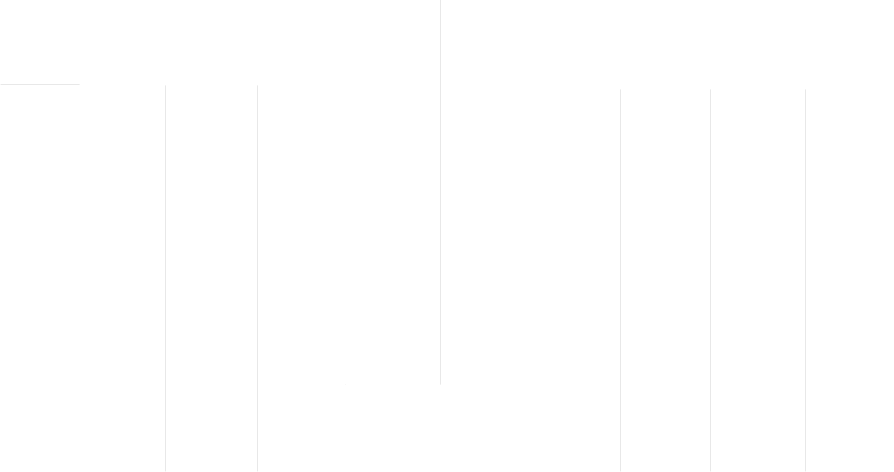
\includegraphics[height=30pt]{AM-logo-TUM-voll-weiss-RGB}};
		\node[black,anchor=west,xshift=32pt,yshift=30pt] at (frame.west) {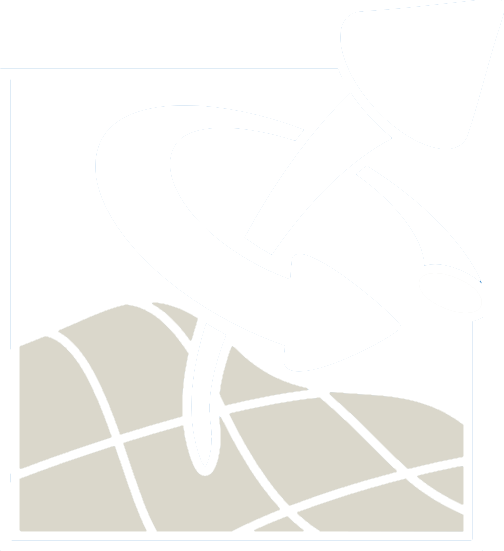
\includegraphics[height=75pt]{AM-logo-AM-ivory-RGB}};
		\node[TUMIvory,xshift=-2cm] at (frame.center) {\bfseries\Huge The \textcolor{white}{AMlatex} GitLab Project};
	},overlay app={%
		\node[opacity=1,xshift=-2.0cm] at([xshift=-3cm]frame.east) {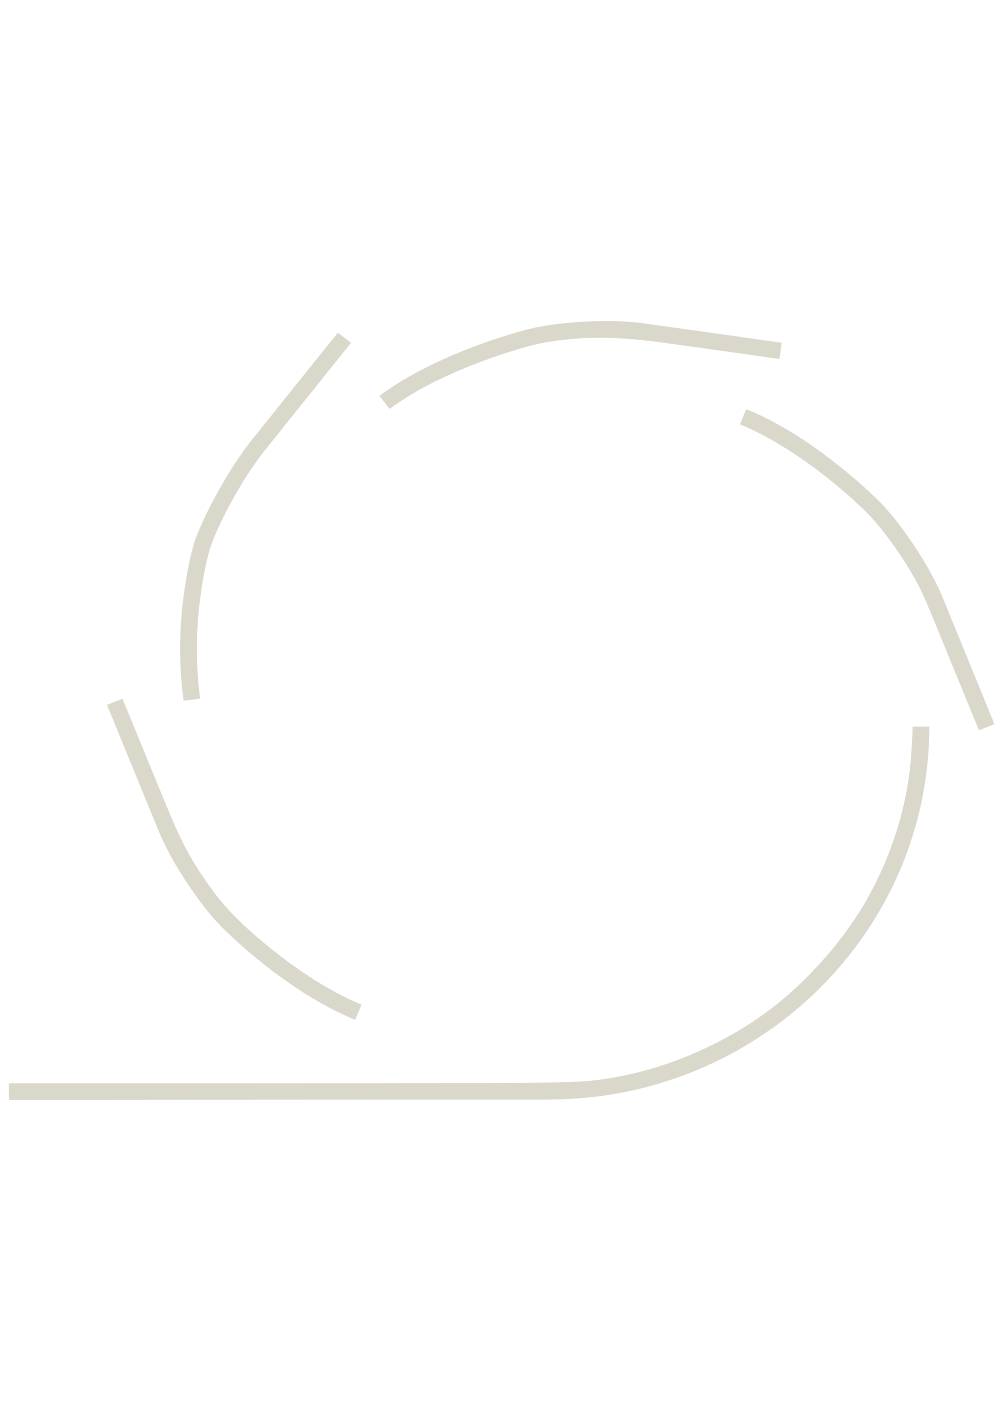
\includegraphics[width=4.5cm]{AM-logo-MW-ivory-RGB}};
	},
]
\end{tcolorbox}
\end{document}